\documentclass[tikz,border=5mm]{standalone}
\usepackage{tikz}
\usetikzlibrary{arrows.meta, positioning, shapes.geometric, calc, patterns, decorations.pathmorphing}

% --- COLOR DEFINITIONS ---
\definecolor{Garnet}{HTML}{73000A}
\definecolor{CBlue}{HTML}{466A9F}
\definecolor{CDark}{HTML}{1F414D}
\definecolor{CGold}{HTML}{A49137}
\definecolor{CGrayLight}{HTML}{E5E5E5}
\definecolor{CGrayDark}{HTML}{555555}
\definecolor{CWhite}{HTML}{FFFFFF}

\begin{document}

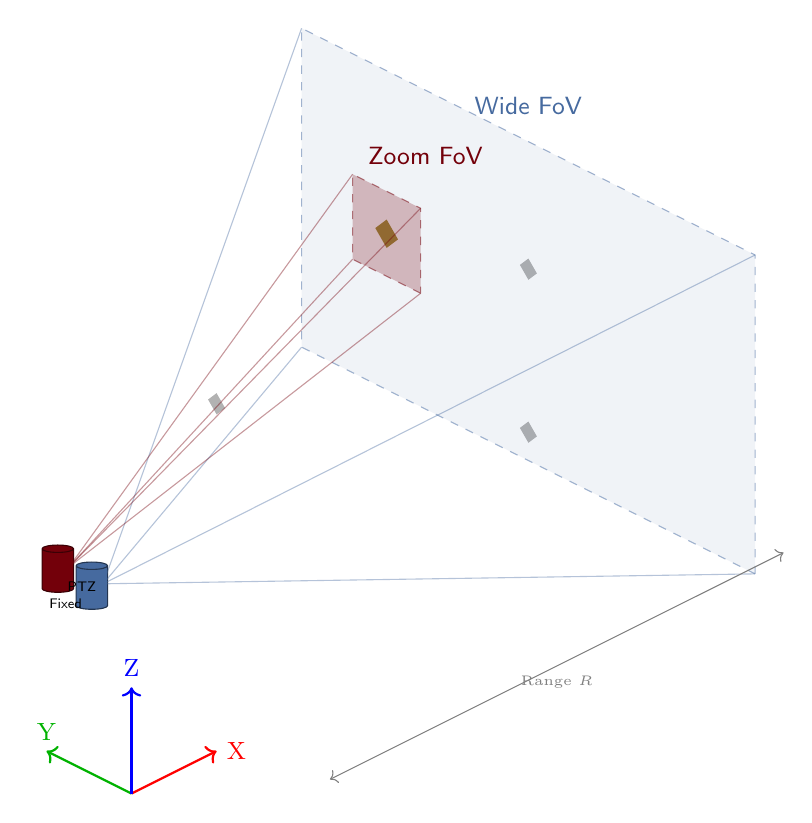
\begin{tikzpicture}[
    x={(0.8cm, 0.4cm)},   % X axis: forward-right
    y={(-0.8cm, 0.4cm)},  % Y axis: forward-left  
    z={(0cm, 1cm)},       % Z axis: up
    scale=0.9
]
    % === COORDINATE AXES ===
    % Draw XYZ axes at a corner for reference
    \coordinate (AxisOrigin) at (-2, -3, -1);
    \draw[->, thick, red] (AxisOrigin) -- ++(1.5, 0, 0) node[right, font=\small] {X};
    \draw[->, thick, green!70!black] (AxisOrigin) -- ++(0, 1.5, 0) node[above, font=\small] {Y};
    \draw[->, thick, blue] (AxisOrigin) -- ++(0, 0, 1.5) node[above, font=\small] {Z};
    
    % === CAMERA POSITIONS ===
    % Both cameras at origin area, side by side along Y axis
    \coordinate (CamFixed) at (0, -0.3, 0);
    \coordinate (CamPTZ) at (0, 0.3, 0);
    
    % Camera icons (vertical cylinders using nodes)
    % Fixed camera (blue) - Solid fill
    \node[cylinder, shape border rotate=90, draw=CBlue!50!black, fill=CBlue, minimum height=0.6cm, minimum width=0.4cm, aspect=0.4, anchor=center] (NodeFixed) at (CamFixed) {};
    % PTZ camera (red) - Solid fill
    \node[cylinder, shape border rotate=90, draw=Garnet!50!black, fill=Garnet, minimum height=0.6cm, minimum width=0.4cm, aspect=0.4, anchor=center] (NodePTZ) at (CamPTZ) {};
    
    % Labels
    \node[below left, font=\tiny\sffamily] at (CamFixed) {Fixed};
    \node[below right, font=\tiny\sffamily] at (CamPTZ) {PTZ};
    
    % === DEFINE GEOMETRY ===
    % Wide FOV geometry
    \def\dist{8}        % Distance to far plane
    \def\wideY{4}       % Half-width in Y at far plane
    \def\wideZup{3}     % Height above horizon at far plane
    \def\wideZdown{1.5} % Height below horizon at far plane
    
    % Wide far plane corners
    \coordinate (WBL) at (\dist, -\wideY, -\wideZdown);  % Bottom-Left
    \coordinate (WBR) at (\dist, \wideY, -\wideZdown);   % Bottom-Right
    \coordinate (WTR) at (\dist, \wideY, \wideZup);      % Top-Right
    \coordinate (WTL) at (\dist, -\wideY, \wideZup);     % Top-Left
    
    % Zoom FOV geometry
    
    \coordinate (Target) at (7, 1.5, 1.5);
    \def\zoomR{0.6}  % Half-size of zoom rectangle
    
    \coordinate (ZBL) at ($(Target) + (0, -\zoomR, -\zoomR)$);
    \coordinate (ZBR) at ($(Target) + (0, \zoomR, -\zoomR)$);
    \coordinate (ZTR) at ($(Target) + (0, \zoomR, \zoomR)$);
    \coordinate (ZTL) at ($(Target) + (0, -\zoomR, \zoomR)$);
    
    % === TARGETS (drawn first so FOV lines appear on top) ===
    % Active target - diamond shape drawn in YZ plane at X=7 (aligned with zoom rectangle)
    \def\tX{7}
    \def\tY{1.5}
    \def\tZ{1.5}
    \def\tS{0.2}  % Size of diamond
    \fill[CGold] (\tX, \tY-\tS, \tZ) -- (\tX, \tY, \tZ+\tS) -- (\tX, \tY+\tS, \tZ) -- (\tX, \tY, \tZ-\tS) -- cycle;
    % Target label removed
    
    % Other objects in wide FOV but outside zoom (diamonds in YZ planes)
    \def\oS{0.15}
    % Object 1 at X=6
    \fill[gray!60] (6, -2-\oS, 0.5) -- (6, -2, 0.5+\oS) -- (6, -2+\oS, 0.5) -- (6, -2, 0.5-\oS) -- cycle;
    % Object 2 at X=5
    \fill[gray!60] (5, 2.5-\oS, -0.5) -- (5, 2.5, -0.5+\oS) -- (5, 2.5+\oS, -0.5) -- (5, 2.5, -0.5-\oS) -- cycle;
    % Object 3 at X=7
    \fill[gray!60] (7, -1-\oS, 2) -- (7, -1, 2+\oS) -- (7, -1+\oS, 2) -- (7, -1, 2-\oS) -- cycle;
    
    % === WIDE FOV (drawn after targets) ===
    % === WIDE FOV (drawn after targets) ===
    % Draw frustum edges from camera front face (offset X by 0.2)
    \coordinate (CamFixedFront) at ($(CamFixed) + (0.2, 0, 0)$);
    \draw[CBlue, thin, opacity=0.4] (CamFixedFront) -- (WBL);
    \draw[CBlue, thin, opacity=0.4] (CamFixedFront) -- (WBR);
    \draw[CBlue, thin, opacity=0.4] (CamFixedFront) -- (WTR);
    \draw[CBlue, thin, opacity=0.4] (CamFixedFront) -- (WTL);
    
    % Far plane rectangle (the "screen")
    \fill[CBlue, opacity=0.08] (WBL) -- (WBR) -- (WTR) -- (WTL) -- cycle;
    \draw[CBlue, dashed, opacity=0.5] (WBL) -- (WBR) -- (WTR) -- (WTL) -- cycle;
    \node[CBlue, font=\sffamily\small] at (\dist, 0, \wideZup+0.5) {Wide FoV};
    
    % === ZOOM FOV (drawn after targets) ===
    % === ZOOM FOV (drawn after targets) ===
    % Draw zoom frustum edges from camera front face
    \coordinate (CamPTZFront) at ($(CamPTZ) + (0.2, 0, 0)$);
    \draw[Garnet, thin, opacity=0.4] (CamPTZFront) -- (ZBL);
    \draw[Garnet, thin, opacity=0.4] (CamPTZFront) -- (ZBR);
    \draw[Garnet, thin, opacity=0.4] (CamPTZFront) -- (ZTR);
    \draw[Garnet, thin, opacity=0.4] (CamPTZFront) -- (ZTL);
    
    % Zoom far plane
    \fill[Garnet, opacity=0.25] (ZBL) -- (ZBR) -- (ZTR) -- (ZTL) -- cycle;
    \draw[Garnet, dashed, opacity=0.5] (ZBL) -- (ZBR) -- (ZTR) -- (ZTL) -- cycle;
    \node[Garnet, font=\sffamily\small, anchor=west] at ($(Target) + (0.5, 1, 0.5)$) {Zoom FoV};
    
    % === ANNOTATIONS ===
    
    % Range
    \draw[<->, gray, thin] (0, -4.5, -1) -- (8, -4.5, -1) node[midway, below, font=\tiny] {Range $R$};
    
\end{tikzpicture}

\end{document}
